\documentclass[a4paper,german,12pt,smallheadings]{scrartcl}
\usepackage[T1]{fontenc}
\usepackage[utf8]{inputenc}
\usepackage{babel}
\usepackage{tikz}
\usetikzlibrary{%
    decorations.pathreplacing,%
    decorations.pathmorphing%
}
\usepackage{verbatim}
\usepackage{geometry}
\usepackage{amsmath}
\usepackage{amssymb}
\usepackage{float}
\usepackage{cancel}
%\usepackage{wrapfig}
\usepackage[thinspace,thinqspace,squaren,textstyle]{SIunits}
\restylefloat{table}
\geometry{a4paper, top=15mm, left=20mm, right=40mm, bottom=20mm, headsep=10mm, footskip=12mm}
\linespread{1.5}
\setlength\parindent{0pt}
\begin{document}
\begin{center}
\bfseries % Fettdruck einschalten
\sffamily % Serifenlose Schrift
\vspace{-40pt}
Elektrodynamik und Optik, Sommersemester 2013, 12. Blatt \\
Markus Fenske, Tutor: Dr. Marko Wietstruk
\vspace{-10pt}
\end{center}
\section*{Aufgabe 1: Ebene elektromagnetische Welle}
\subsection*{Teil a}
\begin{align*}
  f = \frac{\lambda}{c} \approx 300 \;\mega\hertz
\end{align*}

\subsection*{Teil b}
Das elektrische Feld, das magnetische Feld und die Ausbreitungsrichtung stehen
jeweils senkrecht aufeinander. Deswegen Bewegt sich das elektrische Feld in
$x$-Richtung, die Amplitude zeigt in $z$-Richtung.

\subsection*{Teil c}
\begin{align*}
  &|k| = \frac{2 \pi}{\lambda} \approx 6{,}28 \;\meter^{-1} \\
  &\omega = 2\pi f \approx 1884 \;\mega\hertz
\end{align*}

\subsection*{Teil d}

\begin{align*}
  \overline{S} = \frac{1}{\mu_0} \overline{E}\; \overline{B} = \frac{c}{\mu_0} \overline{B}^2 = \frac{cB_{0}^2}{2\mu_0} \approx 119 \;\frac{\watt}{\meter^2}
\end{align*}

\section*{Aufgabe 2: Polarisation}
\subsection*{Teil a}
Die Stäbe des Gitters wirken jeweils als Hertzscher Dipol. Dies bedeutet, dass
in den Stäben eine periodische Spannung induziert wird, die jeweils wieder
elektromagnetische Wellen abstrahlt. Die Schwingungsebene des elektrischen
Feldes ist parallel zu den Gitterstäben, das magnetische Feld steht senkrecht
dazu. Die Schwingungsebene hat sich also geändert und kann damit vom Empfänger
wieder empfangen werden.

\subsection*{Teil b}
Die Energie, die die Stäbe aufnehmen entspricht dem Cosinus des Winkels zum
Sender. Die Energie, die der Empfänger aufnimmt dem Sinus des Winkels. Dies
Gesamtenergie die ankommt ist also proportional zu $\sin\theta \cos \theta$,
die Funktion hat ein Maximum bei $45$ Grad.

\section*{Aufgabe 3: Reflexionsgesetz}
Ist das selbe wie die nächste Aufgabe, nur mit Reflexion statt Transmission und
$c_1 = c_2$, woraus $\alpha = \beta$ folgt. Die Herleitung ist ansonsten
identisch.

\section*{Aufgabe 4: Snelliussches Gesetz}
\begin{figure}[H]
  \begin{center}
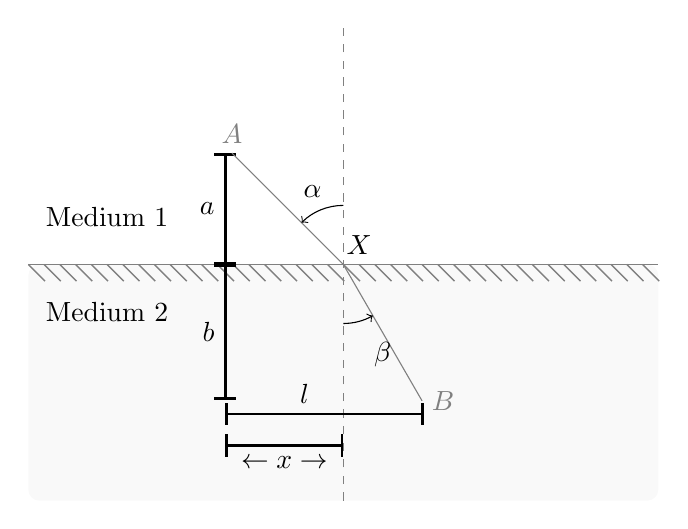
\begin{tikzpicture}[
    media/.style={},
    interface/.style={
        % The border decoration is a path replacing decorator. 
        % For the interface style we want to draw the original path.
        % The postaction option is therefore used to ensure that the
        % border decoration is drawn *after* the original path.
        postaction={draw,decorate,decoration={border,angle=-45,
                    amplitude=0.3cm,segment length=2mm}}},
    ]

    % Round rectangle
    \fill[lightgray!10,rounded corners] (-4,-3) rectangle (4,0);

    % Interface
    \draw[gray,line width=.5pt,interface](-4,0)--(4,0);

    % Vertical dashed line
    \draw[dashed,gray](0,-3)--(0,3);

    % X at center
    \draw(0.2,0) node[above]{$X$};

    % Rulers
    \draw[|-|,line width=1pt](-1.5,0)  -- node[left]{$a$} (-1.5,1.4142);
    \draw[|-|,line width=1pt](-1.5,0)  -- node[left]{$b$} (-1.5,-1.72);
    \draw[|-|,line width=1pt](-1.5,-1.9)  -- node[pos=0.4,above]{$l$} (1.02,-1.9);
    \draw[|-|,line width=1pt](-1.5,-2.3)  -- node[below]{$\leftarrow x \rightarrow $} (0,-2.3);

    % Incidence
    \draw[gray](0:0cm)--(135:2cm) node[above]{$A$};
    \path (0,0)++(113:1cm)node{$\alpha$};
    \draw[->](0,0.75)arc(90:135:.75cm);

    % Transmission
    \draw[gray](0:0cm)--(-60:2cm) node[above,right]{$B$};
    \path (0,0)++(-60:1cm)node[below]{$\beta$};
    \draw[->] (0,-0.75) arc (-90:-60:.75cm);

    % Media names
    \path[media] (-3,.6)  node {Medium 1}
                 (-3,-.6) node {Medium 2};
\end{tikzpicture}
  \end{center}
  \caption{Lichtbrechung beim Übergang zwischen zwei Medien}
\end{figure}

Der Abbilung kann man folgende Gleichung für die Laufzeit in Abhängigkeit der
Position $x$ entnehmen. Es gilt für die Gesamtzeit für die Strecke
$\overline{AX}$ und $\overline{XB}$:

\begin{align*}
  t(x) = \frac{\sqrt{a^2 + x^2}}{c_1} + \frac{\sqrt{(l-x)^2 + b^2}}{c_2}
\end{align*}

Die Funktion soll in Abhängigkeit von $x$ miniert werden.

\begin{align*}
  &\frac{dt}{dx} \overset{!}{=} 0 \\
  \Leftrightarrow\quad&\frac{x}{c_1\sqrt{a^2+x^2}} - \frac{l-x}{c_2 \sqrt{(l-x)^2 + b^2}} \overset{!}{=} 0
\end{align*}

Aus der Zeichnung ist ersichtlich, dass $x = \sqrt{a^2 + x^2} \sin \alpha$ und
$l-x = \sqrt{(l-x)^2 + b^2} \sin \beta$.

\begin{align*}
  \Leftrightarrow\quad&\frac{\sin \alpha}{c_1} - \frac{\sin \beta}{c_2} \overset{!}{=} 0 \\
  \Leftrightarrow\quad&\frac{c_2}{c_1} = \frac{\sin \beta}{\sin \alpha}
\end{align*}

\section*{Aufgabe 5: Totalreflexion}

Siehe vorherige Skizze.

Es gilt das Snelliussche Brechungsgesetz:

\begin{align*}
  \frac{\sin \alpha}{\sin \beta} = \frac{n_2}{n_1}
\end{align*}

Ab einem gewissen Einfallswinkel $\alpha$ wird der Ausfallswinkel $\beta$
größer als $\frac{\pi}{2}$. Ab diesem Punkt passiert eine Totalreflexion, da
der Strahl nicht mehr in das optisch dünnere Medium eintaucht. Wir setzen $\beta = \frac{\pi}{2}$ und lösen nach Einfallswinkel $\alpha$ auf.


\begin{align*}
  &\frac{\sin \alpha}{\sin \frac{\pi}{2}} = \frac{n_2}{n_1} \\
  \Leftrightarrow\quad&\frac{\sin \alpha}{1} = \frac{n_2}{n_1} \\
  \Leftrightarrow\quad&\alpha = \arcsin \frac{n_2}{n_1}
\end{align*}

Sobald also $\alpha > \arcsin \frac{n_2}{n_1}$ passiert Totalreflexion.

\end{document}
